\section{Structure}
The overall structure of our project is as here described, and is illustrated in figure \ref{fig:structure}:
\begin{figure}[h]
    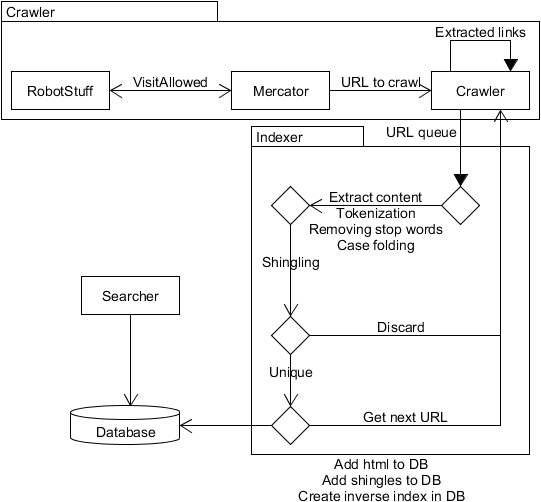
\includegraphics[width=\textwidth]{diagrams/structure}
    \caption{Diagram showing the project structure.}
    \label{fig:structure}
\end{figure}

A crawler instance crawls around, and enqueues downloaded sites for the indexer to use (the crawler acts as a producer, the indexer as a consumer). The crawler feeds itself with new links extracted from the downloaded sites.

An indexer instance dequeues downloaded sites from the queue, and indexes them, saving the information to an MSSQL database.

A searcher instance allows the user to search in the index.

\section{General information}\label{sec:rem-chars}
We only download and index .dk sites. Our implementation is a \emph{little} impolite, as it downloads robots.txt when necessary, resulting in two consecutive hits to the same domain (if the requested URL may be visited).

\subsection{Removed characters}
We remove the characters \texttt{, . ? : "}. This results in some mistakes (e.g. dates), but we deem it acceptable.